\subsection{Требования к функциональным характеристикам}

Программа состоит из двух основных компонент: клиентской и серверной частей, между которыми должно быть налажено
взаимодействие.
В данном документе описаны требования к серверной части.

\subsubsection{Требования к серверной части}
На серверной части должен быть реализован алгоритм по преобразованию единого видеоролика в набор видеороликов меньшей длительности
(сегментов).
Также требуется добавить конвертацию видеоролика в видеоролики с меньшим качеством (Рис.~\ref{ris:server_converting}).

Алгоритм конвертации видеоролика следующий:
\begin{enumerate}
    \item Клиент загружает видеофайл на сервер.
    \item Сервер конвертирует видеофайл в видеофайлы меньших разрешений.
    \[ video1080 \Rightarrow videos = \{ video1080, video720, video480, video360, video240, video144 \} \]
    Данное действие требуется сделать для обеспечения возможности менять качество воспроизводимых роликов в плеере клиента,
    а также для сжатия самих файлов с целью ускорения кэширования видеороликов клиентом.
    \item Сервер разделяет каждый видеоролик из множества видеороликов \(videos\) на небольшие фрагменты (1 сек.).
    \[ video = part1 + part2 + \cdots, \;\;\; video \in videos \]
    Данное действие требуется сделать для обеспечения возможности измененять качество и настройки видео в процессе его воспроизведения
    (без повторного кэширования и приостановки воспроизведения).
\end{enumerate}

Требуется реализовать API для обеспечения взаимодействия сервера с клиентами.
Реализованные методы API и протоколы взаимодействия должны быть задокументированы.

Должно быть реализовано взаимодействие с базой данных для хранения данных о комнатах.

\newpage

\subsubsection{Требования к взаимодействию клиентской и серверной частей}
Взаимодействие между клиентом и сервером должно осуществляться посредством HTTP-запросов и WebSocket-подключений.

При получении HTTP-запроса (GET, POST, UPDATE, DELETE и т.д.) от клиента, сервер должен ответить сообщением в формате
JSON, содержащим необходимую информацию для работы клиента.

Для синхронизации видеопотока между разными клиентами используется протокол WebSocket.
В целях обеспечения наименьшей рассинхронизации видеопотока между клиентами, требуется хранить переменные \(diff\_sc\) и \(diff\_cs\) для
каждого клиента.
Данные переменные будут содержать в себе информацию о количестве затрачиваемого времени при передаче данных от сервера к клиенту или от клиента к серверу.

Формула для определения переменных \(diff\_sc\) и \(diff\_cs\): \begin{gather*}
                                                                    diff\_sc = time\_sc_2 - time\_sc_1\\
                                                                    diff\_cs = time\_cs_2 - time\_cs_1
\end{gather*}, где:
\begin{itemize}[noitemsep]
    \item[--] \(time\_sc_1\) — время отправки сообщения сервером;
    \item[--] \(time\_sc_2\) — время получения сообщения клиентом;
    \item[--] \(diff\_sc\) — разница между временем отправки и временем получения при передаче сообщения от сервера к клиенту;
    \item[--] \(time\_cs_1\) — время отправки сообщения клиентом;
    \item[--] \(time\_cs_2\) — время получения сообщения сервером;
    \item[--] \(diff\_cs\) — разница между временем отправки и временем получения при передаче сообщения от клиента к серверу.
\end{itemize}

Так как возможно подключение нескольких клиентов, требуется хранить содержимое значений \(diff\_sc_i\) и \(diff\_cs_i\) для всех \(n\) клиентов.

Алгоритм (Рис.~\ref{ris:interaction_format}) синхронизации видео единый:
\begin{enumerate}
    \item Клиент \(k\) отправляет серверу запрос на действие \(d\) (перемотку/приостановку/возобновление) видео.
    \item Сервер отправляет всем клиентам сообщение с текущим серверным временем.
    Клиенты принимают значение и считают разницу \(diff\_sc_i\) с учётом своего времени.
    Затем клиенты отправляют посчитанную разницу времени в миллисекундах обратно серверу, а также отправляют текущее клиентское время.
    С учётом полученной информации сервер считает разницу \(diff\_cs_i\).
    \item Сервер отправляет всем клиентам команду выполнить действие \(d\) и передаёт каждому клиенту задержку \(delay_i\),
    которая считается по формуле: \[ delay_i = \max(diff\_sc_1, \ldots, diff\_sc_n) - diff\_sc_i + diff\_cs_k, \;\;\; i \in [1, \ldots, n] \]
\end{enumerate}

Значение \(delay_i\) требуется по-разному использовать в различных ситуациях.
При организации совместного просмотра фильма возможны следующие сценарии:
\begin{itemize}
    \item[--] \textbf{Перемотка} видео на позицию \(t\) мс одним из клиентов.

    При получении такой команды все клиенты (кроме клиента-инициатора) выполняют перемотку видео на позицию \((t + delay_i)\) мс.
    \item[--] \textbf{Приостановка} видео одним из клиентов.

    При получении такой команды все клиенты (кроме клиента-инициатора) приостанавливают воспроизведение и выполняют перемотку видео на \(delay_i\) мс назад.
    \item[--] \textbf{Возобновление} видео одним из клиентов.

    При получении такой команды все клиенты (кроме клиента-инициатора) возобновляют воспроизведение и выполняют перемотку видео на \(delay_i\) мс вперёд.
\end{itemize}

\begin{figure}[p]
    \centering
    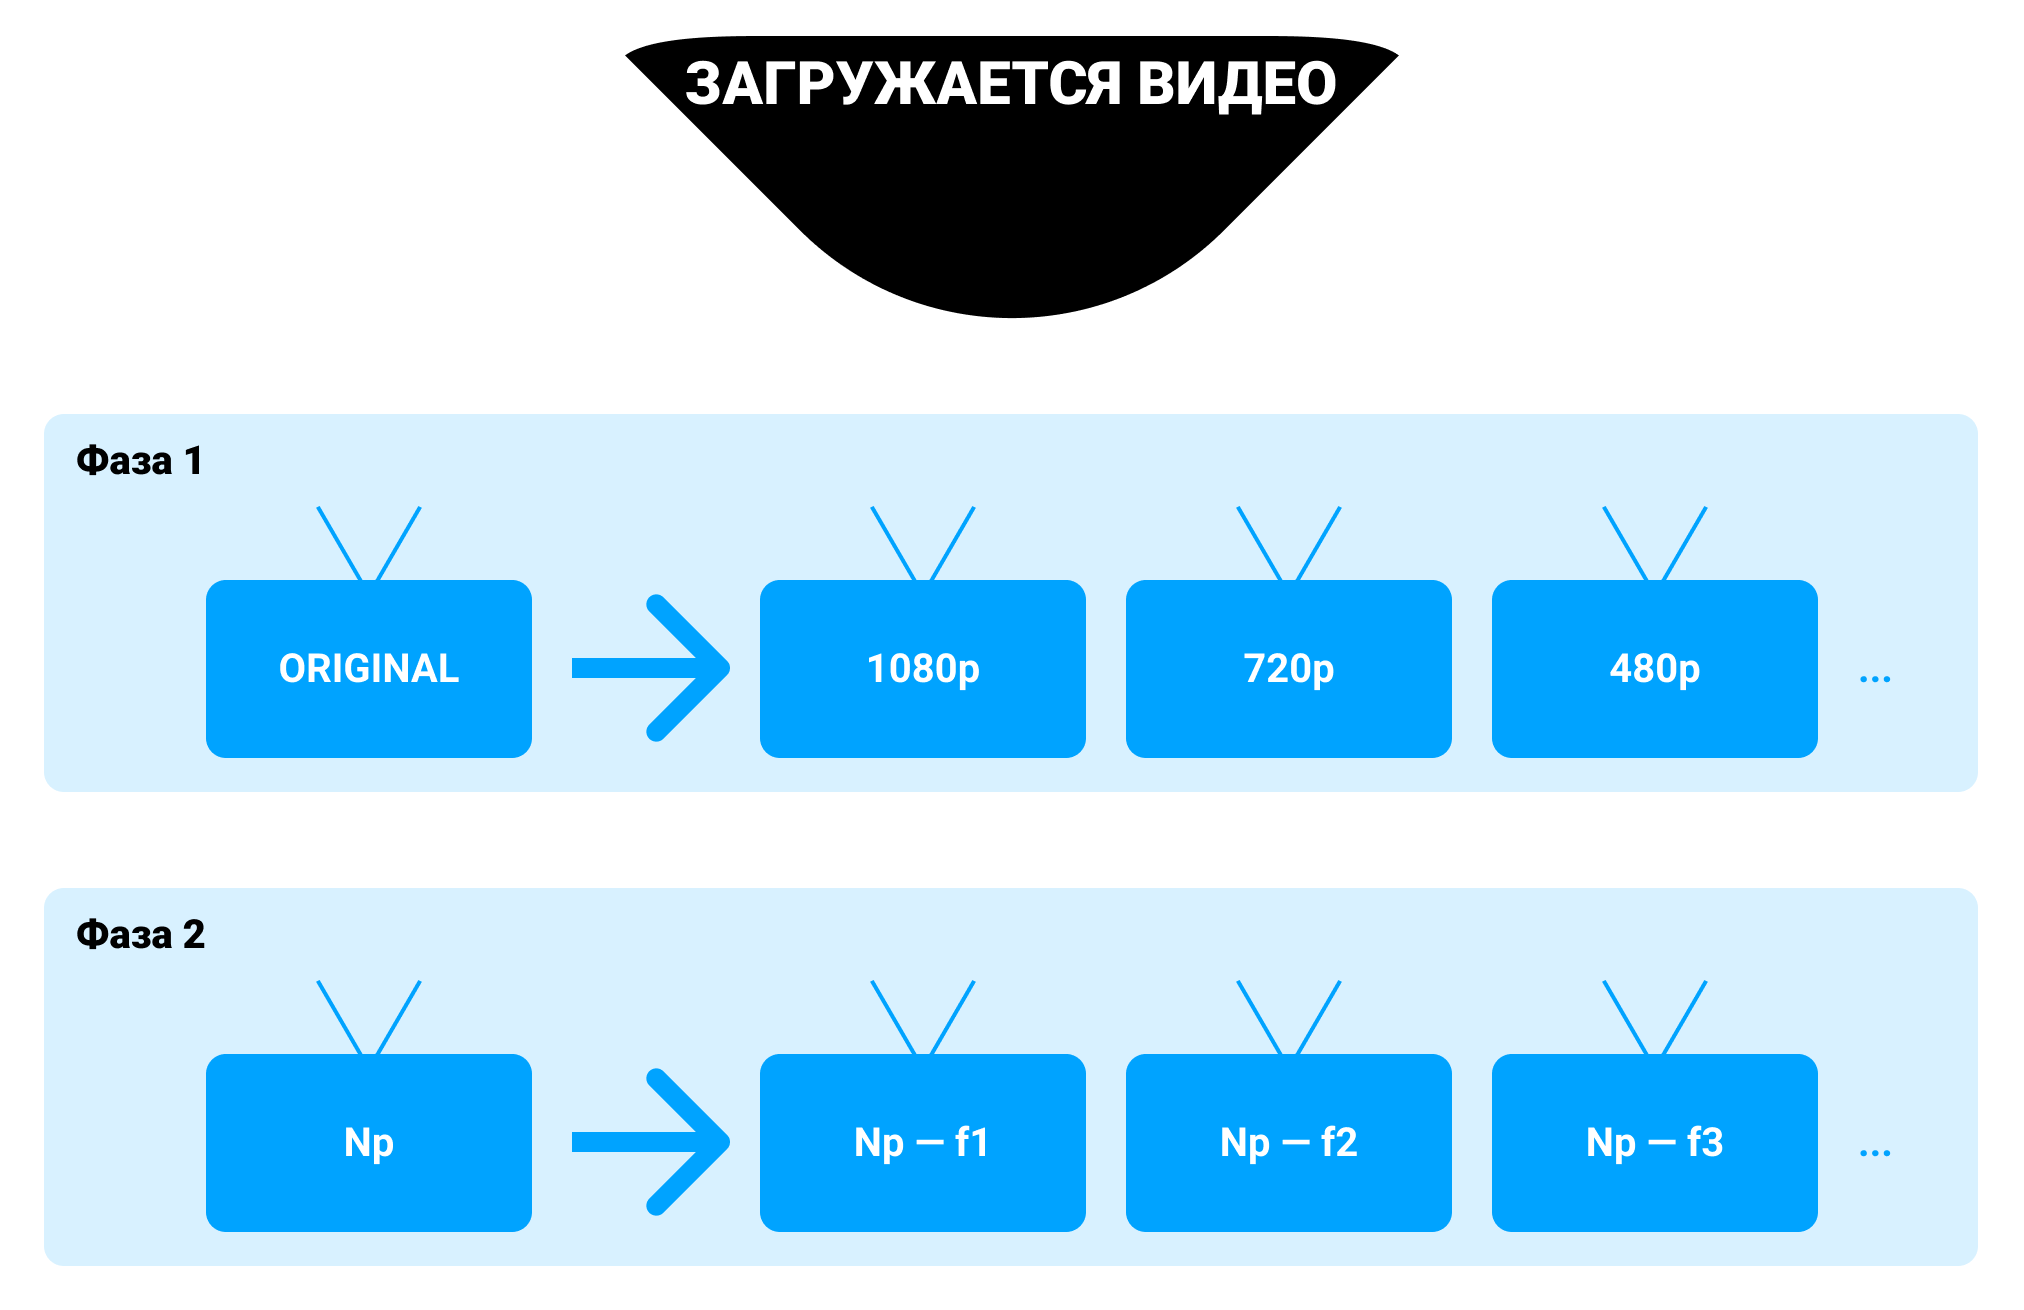
\includegraphics[width=0.97\linewidth]{../images/server_converting.png}
    \caption{Алгоритм конвертации видео}
    \label{ris:server_converting}
\end{figure}

\begin{figure}[p]
    \centering
    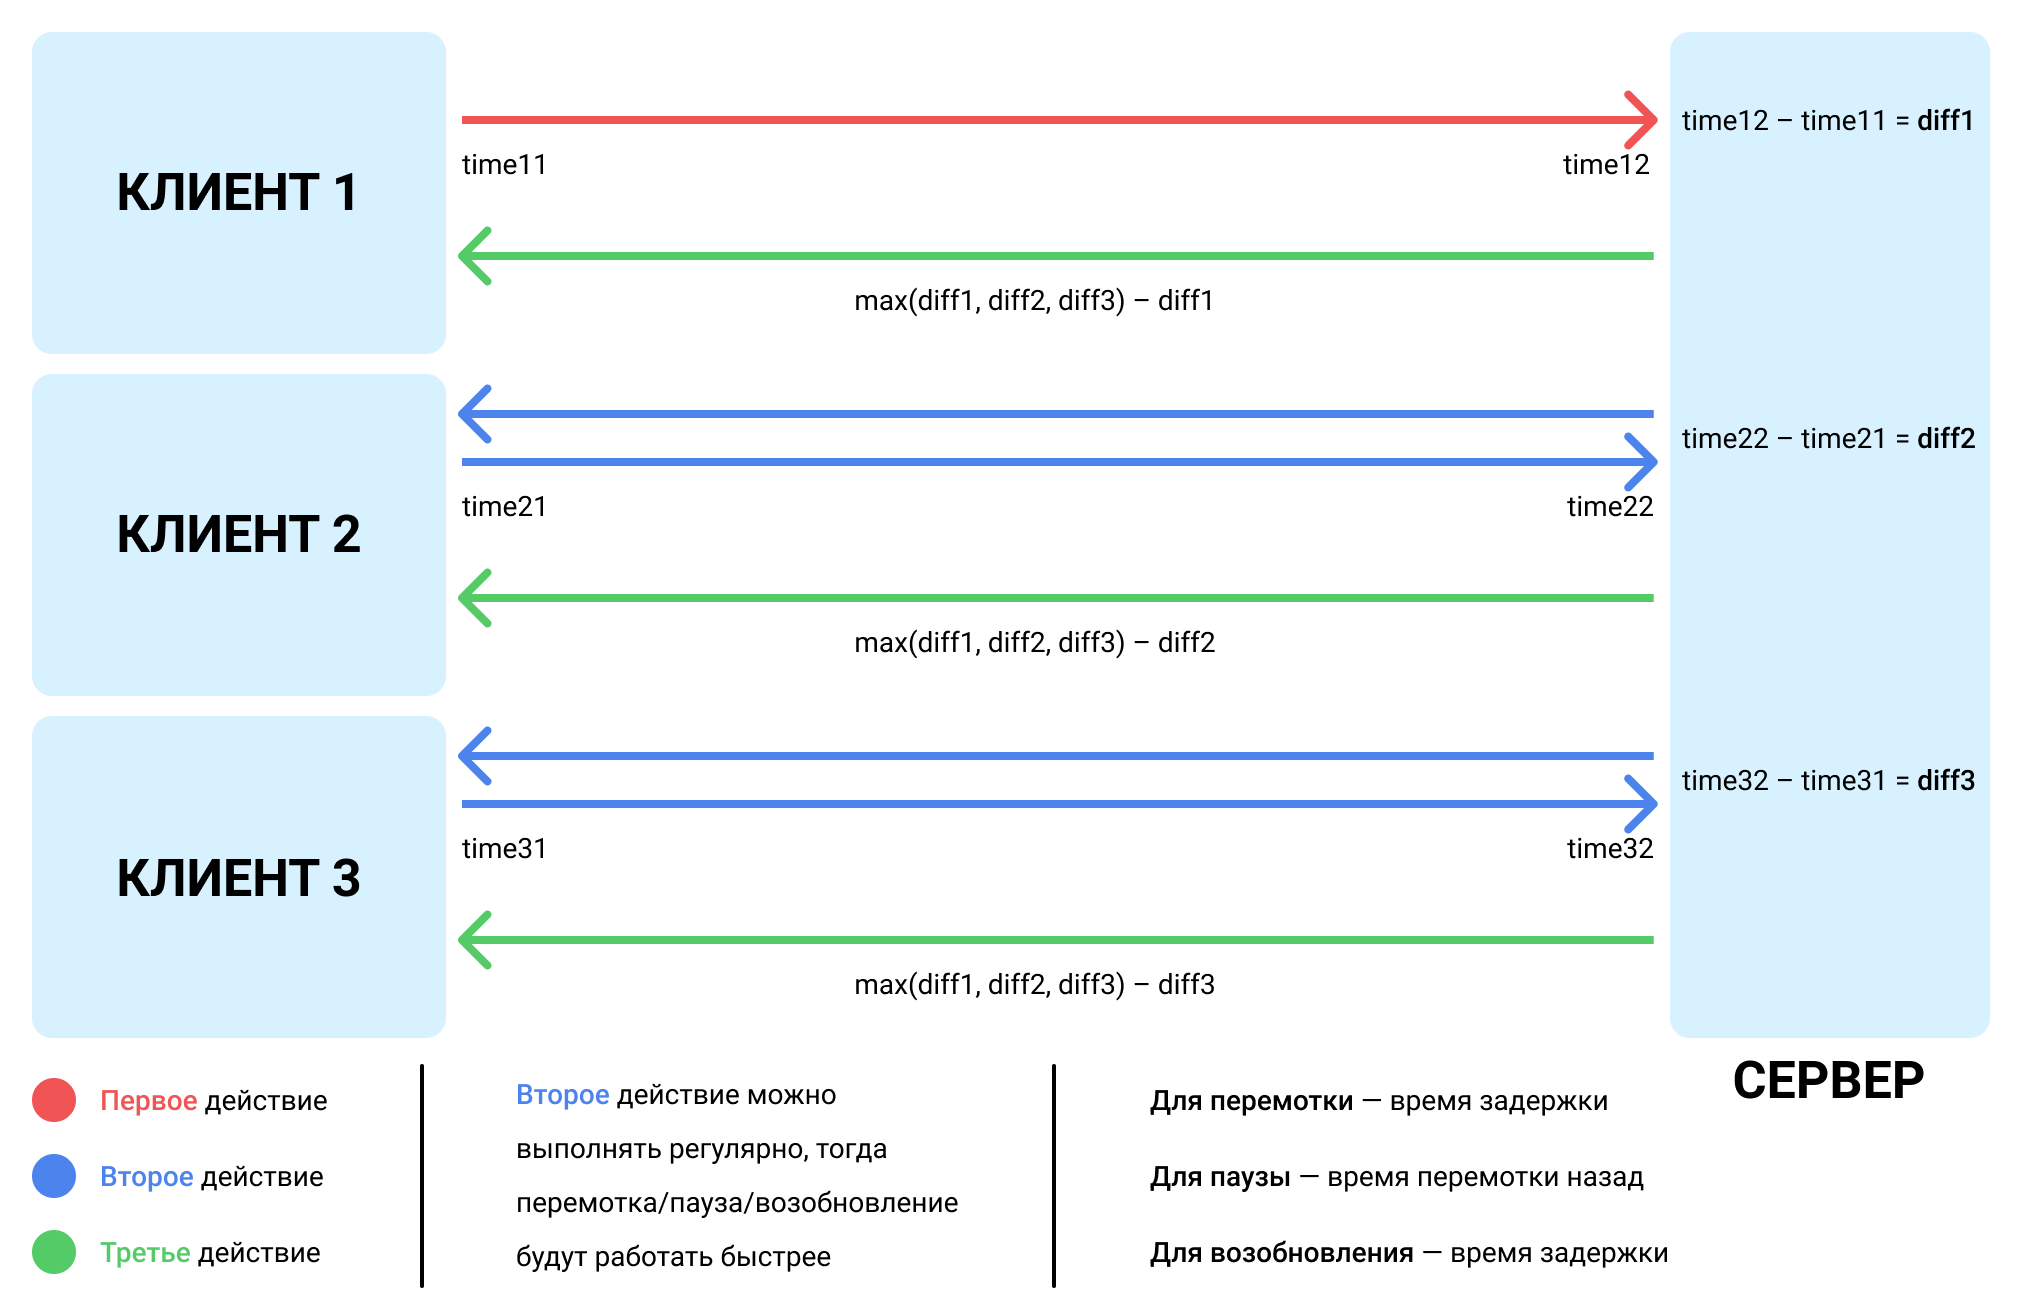
\includegraphics[width=0.97\linewidth]{../images/interaction_format.png}
    \caption{Алгоритм синхронизации видеопотока}
    \label{ris:interaction_format}
\end{figure}

\newpage

\subsubsection{Требования к организации входных данных}
Входными данными для серверной части приложения будут являться:
\begin{enumerate}
    \item HTTP-запросы от клиентской части приложения, которые могут содержать в себе
    тело в формате JSON;
    \item запросы от клиентов с помощью протоколов на базе UDP\@.
\end{enumerate}

\subsubsection{Требования к организации выходных данных}
Выходными данными для приложения будут являться:
\begin{enumerate}
    \item HTTP-ответы на запросы клиентской части, которые будут содержать следующую информацию:
    \begin{enumerate}
        \item код состояния,
        \item тело ответа в формате JSON,
        \item различные заголовки;
    \end{enumerate}
    \item ответы для клиентов с помощью протоколов на базе UDP.
\end{enumerate}